\documentclass[11pt]{article}
\usepackage[T1]{fontenc}
\usepackage[utf8]{inputenc}
\usepackage[margin=1in]{geometry}
\usepackage{amsmath,amssymb,amsthm}
\usepackage{booktabs,longtable,array}
\usepackage{tikz}
\usetikzlibrary{arrows.meta,positioning}
\usepackage{hyperref}
\hypersetup{colorlinks=true,linkcolor=blue,citecolor=blue,urlcolor=blue}
\usepackage{microtype}
\newtheorem{theorem}{Theorem}[section]
\newtheorem{lemma}[theorem]{Lemma}
\newtheorem{proposition}[theorem]{Proposition}
\newtheorem{corollary}[theorem]{Corollary}
\theoremstyle{definition}
\newtheorem{definition}[theorem]{Definition}
\theoremstyle{remark}
\newtheorem{remark}[theorem]{Remark}
\newcommand{\Z}{\mathbb Z}
\newcommand{\N}{\mathbb N}
\newcommand{\dist}{\lVert\,\cdot\,\rVert_\infty}
\newcommand{\A}{\alpha}
\newcommand{\Win}{\operatorname{Win}}
\newcommand{\Succ}{\operatorname{Succ}}
\newcommand{\code}[1]{\texttt{#1}}
\title{A Computer-Assisted Proof of a First-Player Win\\in Infinite Freestyle Gomoku}
\author{Gaoqiang Liu\thanks{Preprint, version 1; not externally peer reviewed. The complete certificate corpus is not yet publicly archived. Artifact availability and verification limitations are stated in Section~\ref{sec:repro}.}\\University of Bayreuth, Bayreuth, Germany\\\href{mailto:Gaoqiang.Liu@uni-bayreuth.de}{\texttt{Gaoqiang.Liu@uni-bayreuth.de}}}
\date{3 October 2026}
\begin{document}
\maketitle
\begin{abstract}
We present a computer-assisted proof that the first player wins freestyle
Gomoku on the infinite integer lattice. Players alternately occupy an empty
lattice point, and a consecutive run of at least five stones in any of four
directions wins immediately; neither player has forbidden moves. The
certified strategy starts at the origin and wins before the second player
within 35 placements in total. The finite proof object uses a conservative
abstraction which truncates adjacent coordinate gaps to five, separately on
the two axes. We prove preservation of winning lines, coverage of every legal
second-player placement, and implementability of relative first-player
actions in every concrete preimage. Thus distant play is represented rather
than treated as a harmless pass. Symmetry reduces the first reply to 20
orbits covering 120 normalized positions. Bounded threat rules compress parts
of the strategy while retaining counterthreats and actual move counts. A
checker independent of the search reconstructs successor sets and checks the
complete dependency closure. We describe the mathematical soundness argument,
the recorded verification, and the requirements for a portable release. The
bound is an upper bound, not an assertion of optimality.
\end{abstract}

\section{Introduction}
\label{sec:intro}
Gomoku is a strong positional game: either player can win by completing a
prescribed line, and the order in which the two players complete their lines
matters. This paper concerns the infinite board, not an extension of the
boundary rules of a finite board. Both players can use every point of $\Z^2$.
In particular, the second player can build a threat outside the region in
which the first player's attack began, force defensive moves, and later
connect stones that were previously separate. A proof must account for all
these possibilities and for a second-player win that occurs first.

The finite-board result is an important computational precedent. Allis,
van den Herik, and Huntjens solved two unrestricted variants on a $15\times15$
board, including the variant in which overlines win
\cite{Allis1993,Allis1996}. Their threat-space search and proof-number search
also suggest how to generate strategy candidates. A finite-board strategy,
however, is not by itself an infinite-board strategy. Additional cells create
additional winning lines for the second player as well as additional legal
replies. A boundary may assist the first player's defensive obligations;
removing it is not a monotone change in the strong game.

Our contribution is a finite, independently checkable proof object for the
infinite freestyle rules. Its central mathematical device is a dynamic
coordinate-gap abstraction. It retains every stone of both colors, records
all small coordinate differences exactly, and uses finite conservative
transition sets for large gaps. A first-player action is specified relative
to an existing stone and is checked against every possible abstract outcome.
The strategy therefore has an interpretation on every actual lattice
position represented by a certificate node. The abstraction need not be an
exact quotient of the game; spurious abstract outcomes are allowed, but all
of them must also have a certified continuation.

The main result is the following.
\begin{theorem}[Infinite freestyle Gomoku]
\label{thm:main}
On $\Z^2$, with Black moving first, alternating placements on empty points,
no forbidden moves, and a consecutive run of at least five stones in one of
the horizontal, vertical, or two diagonal directions winning immediately,
Black has a strategy with first move $(0,0)$ which wins before White against
every legal White strategy. The win occurs after at most 35 actual placements
by the two players combined, counted from the empty board.
\end{theorem}

The proof has two parts. The mathematical part proves that the accepted
certificate rules imply a strategy on the actual infinite board. The
computational part verifies a particular finite certificate satisfying
those rules. The checker does not trust engine evaluations, search success
labels, or omitted branches. The conclusion does not assert that 35 is the
smallest possible uniform bound, nor that every play lasts 35 moves. The
manual soundness argument and conventional program execution are the basis
of this computer-assisted proof; a proof-assistant formalization is not part
of the result.

\subsection{Related work and the scope of the claim}
The literature review distinguishes strong play, where either player may
win first, from weak Maker--Breaker games, in which the second player's
only role is to obstruct the first player. Results for the weak game do not
automatically settle the strong game. Erde's work on a biased $n$-in-a-row
game also uses a different move protocol \cite{Erde2012}. Pairing strategies
for larger targets \cite{Gyorffy2019} concern defensive strategies and a
different target length. Surveys and accounts dated 2014, 2019, and 2022
describe the infinite strong five-in-a-row problem as open
\cite{Hefetz2014,Gyorffy2019,Pluhar2022}. These are dated statements of the
literature, not a claim that an exhaustive search can certify the absence
of all intervening work. We do not use a priority claim as a premise of the
proof.

An additional logical distinction concerns bounded play. A winning strategy
in a general infinitely branching game need not have a uniform finite
winning-time bound merely because each individual play terminates. The
locality result discussed by Hamkins and Leonessi explicitly excludes Gomoku
in its treatment of simple stone-placing games \cite{Hamkins2023}. Our
uniform bound comes from the actual ranks and bounded strategies of the
certificate, not from a compactness assertion about arbitrary Gomoku
strategies.

In particular, the strong-to-weak transfer removes the obligation to stop
the opponent's own line. It does not justify the reverse transfer. The
finite $15\times15$ solution therefore supplies an infinite-board weak-game
precedent, while the present strong-game proof must add the White-first-win
checks. The 35-ply finite principal line described by Allis and coauthors
is likewise distinct from this paper's uniform 35-placement bound against
all actual infinite-board defenses \cite{Allis1993,Hefetz2014}.

\section{Rules and finite positions}
\label{sec:rules}
Let
\[
 D=\{(1,0),(0,1),(1,1),(1,-1)\}.
\]
A five-segment is a set $L=\{s+id:0\leq i\leq4\}$, where $s\in\Z^2$
and $d\in D$. A finite position is a pair $P=(B,W)$ of finite, disjoint
sets of points occupied by Black and White. Write $|P|=|B|+|W|=p$ for
its actual placement count. Reachable nonterminal positions have either
$|B|=|W|$, with Black to move, or $|B|=|W|+1$, with White to move.
A color has won if its set contains a five-segment. This definition includes
all longer consecutive runs because each contains a five-segment.
Every play ends at its first winning placement.

For disjoint $S,T$ with $S$ containing no five-segment, let
\[
 \Win(S,T)=\{q\in\Z^2\setminus(S\cup T):
              S\cup\{q\}\text{ contains a five-segment}\}.
\]
This is the set of immediate winning placements. It is finite for finite
$S$ under the stated nonwinning hypothesis: each such placement completes
a five-segment with four old stones. The notation is also used for virtual
finite positions introduced by threat rules; virtual stones are always
identified as such and do not change the count $p$ of actual placements.
Those uses satisfy the same nonwinning hypothesis. An already winning set
is terminal and is tested directly, not passed to this definition.

The restriction on Black actions in the certificate language is a
restriction on the strategy being certified, not on the game. Black is
legally allowed to play anywhere. It suffices to certify one winning
strategy using a smaller action language. White is subject to no analogous
search restriction: every legal White point must be covered.

\section{Dynamic coordinate gaps}
\label{sec:gaps}
\subsection{Normalization and concrete preimages}
For either coordinate axis, sort the distinct coordinate values of all
points of $B\cup W$, together with the constant anchor $0$:
\[
 v_0< v_1<\cdots<v_m.
\]
If $v_j=0$, define a strictly increasing map $f$ on these values by
\[
 f(v_j)=0,\qquad f(v_{i+1})-f(v_i)=\min(v_{i+1}-v_i,5).
\]
Applying the two maps independently gives the normalization
\[
 \A(P)=\bigl(\{(f_x(x),f_y(y)):(x,y)\in B\},
             \{(f_x(x),f_y(y)):(x,y)\in W\}\bigr).
\]
The anchor is a coordinate convention, not an extra stone. Normalization
retains colors, stone identities, occupancy, turn, and actual placement
count. A normalized position $Q$ represents every $P$ with $\A(P)=Q$.
A normalized adjacent gap equal to five represents any actual adjacent gap
of length at least five. Thus an abstract position generally has infinitely
many concrete preimages.

\begin{lemma}[Exact short coordinate differences]
\label{lem:short}
For any two old coordinate values $u,v$, if $|u-v|\leq4$, then
$f(v)-f(u)=v-u$. Conversely, if $|f(v)-f(u)|\leq4$, then the same equality
holds. If $|u-v|>4$, then $|f(v)-f(u)|>4$.
\end{lemma}
\begin{proof}
Assume $u<v$ and sum the adjacent gaps between them. If their sum is at
most four, every gap is less than five and none is changed. If a gap of
length at least five occurs, its normalized length alone is five, so the
normalized sum exceeds four. If no such gap occurs, the sum is unchanged.
This proves all assertions; the reversed ordering follows by changing
sign.
\end{proof}

\begin{lemma}[Winning-line and occupancy preservation]
\label{lem:five}
Normalization is injective on old points and preserves, in both directions,
the existence of a five-segment of either color.
\end{lemma}
\begin{proof}
Each axis map is strictly increasing, so two different old points remain
different. In a five-segment, every pair has absolute difference at most
four on each axis. Lemma~\ref{lem:short} preserves these signed differences,
including zero differences. Hence the image is a five-segment of the same
direction. Conversely, the signed differences among any five points which
form a normalized five-segment are all at most four, so their actual
differences are exactly those of that segment. The same argument applies
to each color separately. A run longer than five contains a five-segment,
so overlines require no special exception.
\end{proof}

\begin{figure}[ht]
\centering
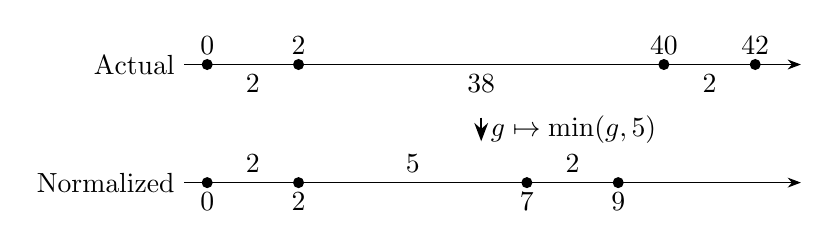
\begin{tikzpicture}[x=0.58cm,y=0.75cm,>=Stealth]
\draw[->] (-0.5,2)--(13,2);
\foreach \x/\lab in {0/0,2/2,10/40,12/42}
 {\fill (\x,2) circle (2pt);\node[above] at (\x,2) {$\lab$};}
\node[below] at (1,2) {2};\node[below] at (6,2) {38};\node[below] at (11,2) {2};
\draw[->] (-0.5,0)--(13,0);
\foreach \x/\lab in {0/0,2/2,7/7,9/9}
 {\fill (\x,0) circle (2pt);\node[below] at (\x,0) {$\lab$};}
\node[above] at (1,0) {2};\node[above] at (4.5,0) {5};\node[above] at (8,0) {2};
\draw[->,thick] (6,1.1)--(6,0.7);
\node[right] at (6,0.9) {$g\mapsto\min(g,5)$};
\node[left] at (-0.5,2) {Actual};\node[left] at (-0.5,0) {Normalized};
\end{tikzpicture}
\caption{One-axis normalization. The upper drawing is schematic, not to scale.
Small gaps remain exact; the gap of length 38 becomes a saturated gap of
length five. The operation is applied to the coordinate values of both
colors and the anchor, not just to the attacking stones.}
\label{fig:gap}
\end{figure}

\subsection{All White placements have finite representatives}
Suppose the old coordinate values are normalized. An inserted coordinate
is equal to an old value, lies outside both extremes, or splits one old
adjacent gap. Equal-value insertions are retained because a point with the
same $x$ or $y$ coordinate need not be occupied. Beyond an extreme, the
distance is represented by one of $1,2,3,4,5$. An exact gap $g<5$ is split
at each integer $u$ with $1\leq u<g$. A saturated gap is split into
truncated parts $(a,b)$ with
\begin{equation}
 \label{eq:split}
 1\leq a,b\leq5,\qquad a+b\geq5.
\end{equation}
For each insertion type, the old values and the new value are renormalized
together, keeping the anchor at zero. Take the Cartesian product of the
two axis insertion sets, transform all old stones, add the new White
stone, and discard occupied targets. Duplicate normalized child states
are merged. Denote the resulting finite set by $\Succ_W(Q)$.

\begin{lemma}[Complete White coverage]
\label{lem:white}
For every preimage $P$ of $Q$ and every legal actual White point $q$,
$\A(B,W\cup\{q\})\in\Succ_W(Q)$.
\end{lemma}
\begin{proof}
On each axis classify the actual new coordinate as above. Equal coordinates
are included. An exterior distance $u$ has type $\min(u,5)$. In an exact
old gap, its length and every possible integer split are unchanged. In an
actual saturated gap $G\geq5$, write the new positive lengths as
$u+v=G$. Their truncations $a=\min(u,5)$ and $b=\min(v,5)$ satisfy
\eqref{eq:split}. The unsplit gaps are unchanged in type, so this insertion
gives exactly the normalized old coordinates and new coordinate obtained
from the actual position. The two axes can be treated independently.
Injectivity ensures that a legal actual target is not removed by the
occupancy filter.
\end{proof}

The converse for a fixed preimage is unnecessary: the finite successor set
may contain extra children. Those children impose extra proof obligations.
They never justify removal of an actual reply. The independent checker
constructs its axis types differently: it realizes an old saturated gap at
every concrete length from five through ten and renormalizes each integer
insertion. This produces the same types as \eqref{eq:split}. Indeed each
such pair has a realization of length $a+b\in[5,10]$, and any larger gap
has one of the same truncated pairs. Unsplit saturated gaps can be realized
at five without changing these local insertion data. This finite enumeration
is accompanied by the argument above; checking a handful of large example
distances alone would not prove coverage of all distances.

\subsection{Implementable Black actions and their uncertainty}
A relative Black action is a pair $(r,\delta)$, where $r$ is an old occupied
point in the normalized position and $\delta\in\Z^2$ satisfies
$\|\delta\|_\infty\leq4$. It designates $r+\delta$, which must be empty in
the normalized position. In a concrete preimage, Black uses the actual
stone corresponding to $r$ and places at $r_{\rm act}+\delta$. Both colors
may provide a reference stone. Only the first move on the empty board has
the special absolute instruction $(0,0)$.

\begin{lemma}[Relative-action legality and coverage]
\label{lem:black}
The designated Black placement is legal in every preimage. Filtering the
complete two-axis insertion types by
$q'_i-f'_i(r_i)=\delta_i$ for each axis $i$ gives a finite set
$\Succ_B(Q,r,\delta)$ which contains every actual normalized outcome of
that placement. All outcomes in this set must be certified.
\end{lemma}
\begin{proof}
An old actual stone occupying $r_{\rm act}+\delta$ has signed differences
$\delta_i$ from the reference, each of absolute value at most four.
Lemma~\ref{lem:short} would place its image at $r+\delta$, contradicting
the checked empty target. Conversely an old image at that target would
give exactly that actual displacement. The action is therefore legal
uniformly. After inserting the actual target, the target--reference
differences are still small and exact, so its axis insertion types pass
the filter. Lemma~\ref{lem:white}'s insertion argument is independent of
the color of the added stone and proves coverage. Filtering can retain
spurious outcomes, which are handled by requiring every retained child.
\end{proof}

An action can have more than one normalized outcome even though the actual
strategy makes a single definite placement. For example, let Black have
$(0,0)$ and let White have $(-60,-G)$, with $G\geq5$. Every such position
normalizes to Black at $(0,0)$ and White at $(-5,-5)$. Place Black at
$(1,-1)$ relative to the origin. If $G=5$, White normalizes to $(-5,-5)$
afterwards; if $G\geq6$, White normalizes to $(-5,-6)$. The gap that was
saturated has been split by the new coordinate. A strategy certificate
must cover both outcomes. A search that keeps only the first displayed
outcome would be unsound.

\begin{figure}[ht]
\centering
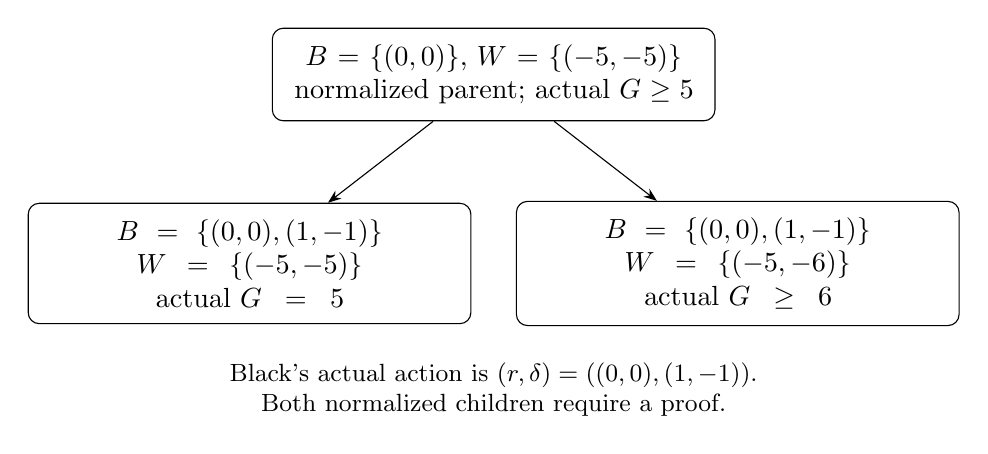
\begin{tikzpicture}[>=Stealth,
 box/.style={draw,rounded corners,align=center,text width=5.2cm,inner sep=6pt}]
\node[box] (root) at (0,0) {$B=\{(0,0)\}$, $W=\{(-5,-5)\}$\\
 normalized parent; actual $G\geq5$};
\node[box] (left) at (-3.1,-2.4) {$B=\{(0,0),(1,-1)\}$\\$W=\{(-5,-5)\}$\\actual $G=5$};
\node[box] (right) at (3.1,-2.4) {$B=\{(0,0),(1,-1)\}$\\$W=\{(-5,-6)\}$\\actual $G\geq6$};
\draw[->] (root)--(left);
\draw[->] (root)--(right);
\node[font=\small,align=center] at (0,-4) {Black's actual action is $(r,\delta)=((0,0),(1,-1))$.\\Both normalized children require a proof.};
\end{tikzpicture}
\caption{A definite actual Black placement can have several abstract outcomes.
This is a geometric example of the certificate's universal outcome
obligation, not a claim that White stones are moved on the actual board.}
\label{fig:black}
\end{figure}

\subsection{Finiteness and the role of distant play}
For an ordinary actual position with $p$ stones, either axis has at most
$p+1$ old coordinate values,
including the anchor. Every adjacent normalized gap is at most five, so
each normalized coordinate lies in $[-5p,5p]$. Thus there are finitely many
normalized colored positions for $p\leq35$, although their number is large. This count concerns ordinary actual
positions; the virtual White unions inside a threat witness do not have
cardinality $p$ and are handled by their separate finite closures.
The certificate selects only a finite subset. Every explicit edge adds
exactly one actual stone, and its placement-count rank strictly increases.

This abstraction retains distant White stones. When further White moves
split their gaps, the resulting children remain among the complete
insertion types. A distant three, a boundary-crossing five, or the later
connection of separate White groups is consequently tested through actual
geometric successor obligations. There is no fixed boundary and no
permission to identify all exterior play with a pass. Remote compression
rules used later require separate sufficient conditions and explicitly
account for defensive interruptions.

\section{Certificate language and soundness}
\label{sec:cert}
\subsection{Explicit nodes and modular files}
An ordinary certificate is a finite directed graph whose nodes record a
normalized colored position, the player to move, and a rule kind. Its
header specifies the freestyle rules and an integer total-placement bound
$H$. We use $H=35$. A nonterminal explicit Black node stores a legal
relative action and an edge to every state of
$\Succ_B(Q,r,\delta)$. A nonterminal explicit White node stores an edge
to every state of $\Succ_W(Q)$. Duplicate child positions are rejected,
and the set of recorded child positions must equal the set reconstructed
by the checker. Every edge increases $p$ by one. The checker rejects
positions with White already winning, and rejects continued play after a
Black win. Terminal nodes must have a Black five, the correct turn parity,
and no White five; they are not accepted merely because a label says
``terminal''.

To keep individual files manageable, a bundle records one such Black or
White node and points to complete child certificates. Each reference
contains the child position, path, and SHA-256 digest of the actual child
bytes. A child must have the stated root and a bound no greater than its
parent's. Missing files, mismatching digests, mismatching roots, incomplete
geometric coverage, and cyclic file references are rejected. Sharing a
completed subproof is permitted. Sharing an unproved search state is not.
Hashes bind data; they do not themselves prove the mathematics.

\subsection{Bounded rules and actual clocks}
Some accepted node kinds stand for a finite winning continuation without
explicitly listing every short reply. For example, after Black has two
distinct immediate winning points, White cannot occupy both in one move;
provided White has no immediate winning placement, Black wins within two
further actual placements. Other rules retain the necessary counterthreat
and blocker replies explicitly. Sections~\ref{sec:short} and
\ref{sec:long} state the sufficient conditions.

A bounded rule at actual count $p$ must provide a strategy valid for every
actual preimage and every subsequent legal White move. It must rule out
White winning first at every intermediate turn and bound the number of
further actual placements by $h$, with $p+h\leq H$. The count $h$ includes
both colors, defensive interruptions, and the move on which Black wins.
A virtual union of possible White defense points is only a conservative
simulation state. Adding three virtual points to that union does not mean
that White made three actual moves, nor that White made zero moves.
Termination is established using the actual strategy clock.

\begin{theorem}[Certificate soundness]
\label{thm:sound}
Assume every bounded rule used by a finite accepted certificate has the
uniform preimage soundness property just described. A certificate rooted
at normalized $Q$ with total bound $H$ supplies an actual Black winning
strategy from every nonterminal preimage $P$ of $Q$, in at most $H-|P|$
further actual placements. Black wins before White.
\end{theorem}
\begin{proof}
Use induction on $H-p$. At an accepted Black terminal, winning-line
preservation gives a Black five in the actual position and excludes a
White five. A bounded-rule node supplies the claimed actual strategy
directly, within its checked clock. At an explicit Black node, the relative
action is legal in every preimage by Lemma~\ref{lem:black}. Its actual
normalized result is one of the certified children; apply induction with
one smaller remaining count. At an explicit White node, whatever legal
point White chooses, Lemma~\ref{lem:white} puts the result among the
children. Each certified child excludes a White win by
Lemma~\ref{lem:five} and has smaller remaining count. Symbolic White rules
partition replies into explicitly covered children and uniformly bounded
winning continuations, so the same argument applies. A symmetry frame,
when used by a rule, transports all actual placements by its checked
lattice isometry and transports them back without changing the clock.
Finite ranks preclude an infinite explicit path. Bundle references are
the same induction across file boundaries, with roots and bounds checked
and file cycles excluded. Therefore all actual plays terminate in a
Black win within the stated bound.
\end{proof}

The soundness theorem separates the universal mathematical statement from
the finite computation. It is not a statement that a heuristic search
which returns success must be correct. Only a fully accepted certificate
can instantiate the theorem. UNKNOWN, timeout, untried actions, incomplete
branches, and candidate proofs cannot instantiate it.

\section{Short threat rules}\label{sec:short}
In this section $\Win(X,Y)$ is used only when $X$ has no five. The normalization map is $\A$; the exhaustive one-move lifting result established earlier routes actual replies to normalized children.

For a full position after $p=|B|+|W|$ actual moves with total limit $H$, every rule that omits a continuation of at most $c$ moves must satisfy $p+c\le H$. The short rules below use $c=2$ or $c=4$ as stated.

\begin{lemma}[rigid old components]\label{mac:rigid-frame}
Form the graph on all old occupied points, including White connector stones, with an edge whenever the Chebyshev distance is at most 4. Each connected component has the same relative coordinates in every integer preimage, and hence moves as a rigid frame under its own translation. No gap displayed as 5 lies strictly within the axis projection of a component. Distinct components can have different translations and must not be treated as one rigid frame.
\end{lemma}
\begin{proof}
By Lemma~\ref{lem:short}, both signed coordinate differences of every edge are exact in every preimage. Summing these displacement vectors along a connected path fixes the difference between any two vertices of its component. If a gap displayed as 5 lay inside a component's axis projection, a path between vertices on opposite sides would have an edge crossing that gap. That edge would have axis difference at least 5, contrary to its Chebyshev distance being at most 4.
\end{proof}

All propositions in this section concern a nonterminal position with White to move. Every retained critical move is sent to every abstract successor of its anchored action. Soundness of this routing uses the exhaustive one-move dynamic-gap transition lemma; the geometric arguments below explain why replies outside the listed actions can be omitted. A chosen action is an old occupied reference point plus an offset of Chebyshev norm at most 4. Different preimages may produce different normalized children, and all those children are required.

\subsection{Immediate completion rules}

\begin{proposition}[double completion]\label{mac:double-completion}
If White has no immediate winning move and Black has at least two distinct immediate winning points, Black wins within the next two actual moves.

\end{proposition}
\begin{proof}
White cannot win on its present move. It occupies at most one of Black's two points. Black occupies another on its next move and wins. Both five-cell witnesses lift by Lemma~\ref{mac:rigid-frame}. This proves both rule labels \texttt{double\_immediate\_win} and \texttt{double\_open\_four}; the labels do not supply additional hypotheses. 
\end{proof}

\begin{proposition}[next-turn finish and exhaustive critical completion]\label{mac:finish-critical}
Suppose that for every legal White move its child has no White five and at least one Black immediate winning point. Black wins within two actual moves. More generally, retain precisely the White children without a Black immediate winning point, verify their continuations, and require no White five in every child. Every omitted child is won by the same two-move argument.

\end{proposition}
\begin{proof}
The chosen White child is exhaustive under one-move lifting. White has not won, and the Black completion witness in that child lifts to the actual board. Black then wins. The second statement applies this argument to each omitted child and uses the verified continuation for each retained one. These are \texttt{next\_turn\_finish} and \texttt{white\_critical}. 
\end{proof}

\begin{proposition}[the small-count open-four critical rule]\label{mac:small-open-four}
Suppose the parent has exactly three Black stones and two White stones. Enumerate all White children, retaining those that contain no template consisting of four consecutive cells with exactly three Black stones, one empty setup point, and both adjacent endpoints empty. Every omitted child is won within four actual moves from the parent.

\end{proposition}
\begin{proof}
In an omitted child White has three stones. Black fills the setup point, giving four consecutive Black stones with two empty winning endpoints. On its next move White has at most four stones in total, so it cannot form five anywhere. White can occupy at most one of the two endpoints, and Black wins at the other. Counting the parent's White reply, Black setup, White reply, and Black finish gives four moves. The exact count \((|B|,|W|)=(3,2)\) in \texttt{white\_open\_four\_critical} is essential to this proof: a template alone in a position with more White stones does not exclude an intervening White win. 
\end{proof}

\subsection{Counterthreat actions and a forced block}

Let \(\mathcal A_W\) contain, for every five-cell segment disjoint from \(B\) and containing exactly three old White stones, every empty point of that segment as an anchored move. Require that every unblocked segment containing at least three old White stones has exactly three; equivalently, the reconstruction rejects any White immediate winning point and any White five. The union of these actions is \texttt{threat\_actions}.

\begin{lemma}[all relevant White counterthreats]\label{mac:counter-actions}
Under these hypotheses White cannot win immediately. If a White move creates any White immediate winning point, that move belongs to \(\mathcal A_W\).

\end{lemma}
\begin{proof}
An immediate White win would require four old White stones in an unblocked five-cell segment, excluded by the hypothesis. A newly created White winning point has a five-cell witness containing four White stones after the move. It must contain the new stone, since the old position has no White winning point, and therefore contains three old White stones. The reconstruction enumerates its new point. The three old stones have span at most 4 in each axis, so the segment is a rigid witness and the enumerated anchored action covers its move in every preimage. 
\end{proof}

\begin{proposition}[forced block]\label{mac:forced-block}
If White has no immediate winning point and Black has an immediate winning point \(q\), retain the anchored White action at \(q\). Every other White reply loses within two moves.

\end{proposition}
\begin{proof}
White cannot win now. A reply away from \(q\) leaves the Black completion at \(q\) available. A supporting Black stone adjacent to the hole exists in any four-of-five witness; using such a stone as reference gives the offset of norm at most 1 used by \texttt{white\_forced\_block\_symbolic}. The completion and anchored block both lift exactly. 
\end{proof}

\subsection{The fork rule}

For each point \(s\), collect targets \(T_s\): a target \(t\ne s\) is included when an unblocked five-cell segment contains exactly three old Black stones and has the two empty points \(s,t\). Choose any \(s\) with at least two distinct targets. If \(|T_s|=2\), the fork blockers are \(\{s\}\cup T_s\); if \(|T_s|\ge3\), the sole necessary blocker is \(s\). Add these blockers to \(\mathcal A_W\). The reference module chooses one such fork; optimality of that choice is irrelevant.

\begin{lemma}[fork witnesses share a rigid frame]\label{mac:fork-frame}
All supporting Black triples of a reconstructed fork belong to one old rigid component, and all their displayed setup points represent the same point of that frame in every preimage.

\end{lemma}
\begin{proof}
A supporting triple consists of three cells of a five-cell segment other than \(s\). At most two cells of that segment lie at distance greater than 2 from \(s\), so the triple has a stone at Chebyshev distance at most 2 from \(s\). Choose one such stone from each triple. Any two chosen stones have mutual distance at most 4, and are joined in the old-stone graph. Each triple is itself connected because its stones lie in one five-cell segment. Thus all triples lie in the same component. Their offsets to the common displayed \(s\), and to each target, are exact within that component, proving the claim. 
\end{proof}

\begin{proposition}[symbolic fork]\label{mac:fork}
Every White move outside the reconstructed blockers and \(\mathcal A_W\) loses within four moves from the parent.

\end{proposition}
\begin{proof}
By Lemma~\ref{mac:counter-actions} the reply neither wins immediately nor creates a White completion point. The setup \(s\) remains empty. If there are two targets, both survive because the reply avoided \(s\) and both targets. If there are at least three targets, a reply away from \(s\) can occupy at most one target and leaves at least two. Black plays \(s\), obtaining two distinct completion points. Adding a Black stone cannot create a White winning point. White therefore cannot win on its next move, and Black completes at a surviving target. Lemma~\ref{mac:fork-frame} establishes this construction in every preimage. This proves \texttt{white\_fork\_symbolic}, with the four-move budget including the initial White reply. 
\end{proof}

\subsection{The open-four template rules}

An open-four preparation template consists of a four-cell segment with exactly three Black stones and one empty setup \(s\), and with both adjacent endpoints \(\ell,r\) empty. Its \textbf{obstruction set} is \(T=\{s,\ell,r\}\). A White reply disables this particular preparation only by occupying \(T\), because its other required cells already contain Black stones. For a nonempty selected family of templates in a common rigid frame, let \(K=\bigcap T\). Retain \(\mathcal A_W\) and the anchored White moves at all points of \(K\).

\begin{proposition}[a selected template family]\label{mac:template-family}
Every White reply outside those retained actions loses within four moves.

\end{proposition}
\begin{proof}
A reply outside \(K\) misses the obstruction set of at least one selected template. Its setup and both endpoints remain empty. By Lemma~\ref{mac:counter-actions} the reply has no immediate or next-turn White win. Black fills that setup. It produces two Black completion points and can only reduce White's completion set. The next White move cannot win or block both endpoints; Black wins on the following move. Each template's support and endpoints lift within the selected rigid frame. 
\end{proof}

The four implementations select justified families as follows.

\begin{itemize}
\item \texttt{white\_open\_four\_symbolic}: if there are at most four Black stones, select all templates. Each uses a three-element subset of \(B\), so any two supporting triples share at least two Black stones and belong to one rigid component. If there are more than four Black stones, select a single template. In either case the selected frame is rigid. A common obstruction point belongs to the first template and is within distance 4 of any supporting stone chosen there as reference.
\item \texttt{white\_open\_four\_symbolic\_shared}: require at least five Black stones and select a family whose templates all contain a chosen old Black supporter. Their offsets are exact from that common supporter. The common obstruction points lie within distance 4 of it.
\item \texttt{white\_open\_four\_symbolic\_component}: require at least five Black stones, form the old-stone components including White connector stones, and select all templates supported in one component. Their offsets are exact by Lemma~\ref{mac:rigid-frame}. Anchor common obstruction points at a supporter of the first selected template, so their offsets have norm at most 4.
\item \texttt{white\_open\_four\_symbolic\_far}: require at least six Black stones and two templates with supporting stones \(u,v\) at displayed Chebyshev distance greater than 8. Each template's obstruction points are within distance 4 of every one of its supporters. If the two obstruction sets shared a point, the triangle inequality would give distance at most 8 between \(u,v\), a contradiction. Coordinate expansion cannot reduce either axis separation between old points; the two sets remain disjoint in every preimage. Every White reply therefore leaves one preparation intact. Only \(\mathcal A_W\) needs retention. The two templates can use separate rigid frames; this argument does not require their relative translation to be known.

\end{itemize}
All these rules use the four-move clock of Proposition~\ref{mac:template-family}. The chosen family and fork may be changed by one of the eight square symmetries. These symmetries preserve legal moves, winning directions, distances, templates, and budgets; applying and then undoing the chosen frame does not alter the proof.

\section{Long threat sequences and remote interruptions}\label{sec:long}
Throughout the local simulation, $A$ denotes a simulated Black set and $D$ denotes a virtual White upper set, not a set of directions. The winning directions remain those fixed in the board rules. All real boards are subsets of $\Z^2$, and normalized full-board successors use $\A$.

For a Black-to-move full root after $p=|B|+|W|$ actual moves, let $h=H-p$ be its remaining budget. The cardinality of a virtual White upper set does not replace $p$: adding every defense of one operator counts as one actual White turn. Local subboards and virtual boards need not have equal Black and White cardinalities.
\subsection{Local operators and their complete sufficient continuation}\label{mac:local-section}

The following is an intrinsic description of the finite checks, independent of whether a program accepts them. Fix a rigid local frame. A step records a Black gain \(g\), required Black support \(R\), an empty set \(U\) containing \(g\), a White defense set \(K\), and one of the following line patterns. Coordinates in the table are consecutive indices along any winning direction; translating a pattern, reversing its line, and choosing any stone of its final Black shape as the gain are allowed. The remaining shape stones are the required support.

\begin{center}
\small
\renewcommand{\arraystretch}{1.25}
\begin{tabular}{@{}lcc@{}}
\hline
Pattern & Black shape after the gain & Defense set $K$ \\
\hline
\texttt{five} & $\{0,1,2,3,4\}$ & $\varnothing$ \\
\texttt{four} & $\{0,1,2,3,4\}\setminus\{t\}$ & $\{t\}$ \\
\texttt{straight\_four} & $\{1,2,3,4\}$ & $\{0,5\}$ \\
\texttt{three} or \texttt{broken\_three} & $\{1,2,3,4\}\setminus\{t\}$ & $\{0,5,t\}$ \\
\texttt{open\_three} & $\{2,3,4\}$ & $\{1,5\}$ \\
\hline
\end{tabular}
\par\medskip
\begin{tabular}{@{}lc@{}}
\hline
Pattern & Required empty cells before the gain \\
\hline
\texttt{five} & $\{g\}$ \\
\texttt{four} & $\{g,t\}$ \\
\texttt{straight\_four} & $\{g,0,5\}$ \\
\texttt{three} or \texttt{broken\_three} & $\{g,0,5,t\}$ \\
\texttt{open\_three} & $\{g,0,1,5,6\}$ \\
\hline
\end{tabular}
\end{center}

In the fourth row the endpoint omissions \(t=1,4\) receive the first label and interior omissions \(t=2,3\) the second. These names have no logical force beyond their reconstructed pattern.

\begin{lemma}[a reply outside a defense set]\label{mac:operator-reply}
After a legal nonterminal gain, assume White has no immediate winning point. An ensuing White reply outside \(K\), which creates no White immediate winning point, loses within two moves for \texttt{four} and within four moves for one of the three-stone types. A \texttt{straight\_four} is won within two moves against every White reply. A \texttt{five} ends immediately at the gain.

\end{lemma}
\begin{proof}
For \texttt{four}, the reply misses the sole completion. For \texttt{straight\_four}, it misses at least one of the two endpoints. For \texttt{three} and \texttt{broken\_three}, Black fills \(t\), giving four consecutive stones with endpoints 0 and 5 free. For \texttt{open\_three}, Black can extend at 1 or 5. Extension at 1 requires endpoints 0 and 5, and extension at 5 requires endpoints 1 and 6. A reply outside \(\{1,5\}\) may occupy 0 or 6, but one stone cannot occupy both; choose the extension whose external endpoint remains free. In each three-stone case this next Black move makes a straight four. The preceding White reply created no White completion, and adding a Black stone cannot create one, so White cannot win on the intervening move. Black then finishes at a remaining endpoint. The counts include the White reply under discussion. 
\end{proof}

The finite local continuation maintains a state \((i,A,D,u)\), with step index \(i\), simulated local Black set \(A\), virtual White upper set \(D\), and actual-move count \(u\). The following conditions define a valid local witness.

\begin{enumerate}
\item Initially \(A,D\) are the old local stones and \(u=0\). At every step \(D\) has no five, the required support lies in \(A\), and the required empty set avoids \(A\cup D\). Add \(g\) to \(A\) and increase \(u\) by one. If Black has five, terminate this branch. Otherwise require \(\Win(D,A)=\varnothing\).
\item A \texttt{straight\_four} terminates this branch with total bound \(u+2\). For the other nonterminal types form a closure of all counterfour responses described below, starting with the state just after the gain.
\item At every White-decision closure state \((A,D,v)\), require that $D$ has no five and \(\Win(D,A)=\varnothing\). For a three-stone operator, enumerate every empty point \(q\) of every five-cell segment disjoint from \(A\) with at least three White stones in \(D\). Put \(D'=D\cup\{q\}\). The prestate conditions imply that $D'$ has no five, since otherwise $q$ was a completion of $D$. If \(\Win(D',A)\) is nonempty, require it to be the singleton \(\{t\}\). Require \(q,t\) to avoid every gain, required support, defense point, and required empty point in the current and later operators. Add the full closure successor \((A\cup\{t\},D',v+2)\). No such response is ignored. A branch whose Black block already makes five may be treated as having terminated early.
\item At every closure state check \(K\cap A=\varnothing\) and that \(D\cup K\) has no five. Append the next step with virtual set \(D\cup K\) and count \(v+1\). Also include the quick-finish bound \(v+4\) for a three-stone type, or \(v+2\) for \texttt{four}.
\item Every branch has a terminal gain or straight four before the sequence runs out. All closure states and all bounds are finite and within the stated local budget. A resource limit, missing step, extra completion point, collision, or excess budget invalidates the witness; a closure may not be truncated and then certified.

\end{enumerate}
Call the maximum of these branch and quick-finish counts \(L\). Let \(E\) contain all old local stones, every operator position, and every position added by any closure edge. Let \(\mathcal P\) be the recorded local states: the initial state, states after gains, states after counterfour blocks, and states after adding virtual defense sets. A local White counterfour state before its Black block is not in \(\mathcal P\); both new move points nevertheless lie in \(E\).

\begin{lemma}[completeness of a local counterfour closure]\label{mac:local-counter}
The enumeration covers every actual local counterfour on any sustained branch represented by \(d\subseteq D\). An accepted virtual closure does not omit a response because a virtual defense already occupies the actual new point.

\end{lemma}
\begin{proof}
At a White decision the accepted virtual state has neither a White five nor a White completion. Suppose an actual legal reply \(q\) creates a White completion \(t\), witnessed by a five-cell segment \(S\). Before \(q\), the segment has three actual White stones and no actual Black stone, so its three-stone support is contained in \(D\) and the enumeration includes \(q\), provided \(q\notin D\).

If \(q\in D\), then \(D\) already contains the resulting actual four-stone support. If \(t\in D\), it already contains a five; otherwise \(t\) is a virtual White completion. Both contradict the accepted prestate. Thus \(q\notin D\). Likewise an actual completion \(t\) cannot be hidden by virtual occupancy: if \(t\in D\), the prestate has four stones of \(S\), missing only \(q\), and hence a virtual completion at \(q\). Therefore the actual completion points persist among the virtual completion points after \(q\). The virtual set must have exactly one completion point, so this point is also the unique actual completion and the prescribed Black block is correct. The virtual post-reply cannot already have five, because this would require a virtual completion in the prestate. The suffix exclusion preserves the current operator and every later recorded requirement. 
\end{proof}

\begin{proposition}[local witness soundness]\label{mac:local-witness}
On the local board a valid witness gives a Black strategy that wins before White within \(L\) actual moves.

\end{proposition}
\begin{proof}
Maintain actual local Black stones equal to \(A\), actual White stones contained in \(D\), and the indicated actual clock. A prescribed Black gain is legal because its empty set avoids the stronger set \(A\cup D\). If it makes five, the actual game ends. At each ensuing White decision an actual immediate win is excluded: its four old stones would give either a five or a completion in the virtual state.

If White occupies \(K\), add all of \(K\) to the virtual set and count one actual White move. The next prescribed Black gain is legal under this stronger set; if that defense gave an actual completion threat, the checks after that gain ensure it is blocked before White moves again. If White instead makes a counterfour against a three-stone operator, Lemma~\ref{mac:local-counter} prescribes its unique block, counts two moves, and returns to the same operator. For \texttt{four} or \texttt{straight\_four}, a White move that merely creates its own four loses to Black's already available five on the next move and does not require a counterfour detour. Every other reply is the quick-finish case of Lemma~\ref{mac:operator-reply}. These cases exhaust all legal White replies. A quick-finish branch ends and never returns to the sequence. The finite continuation conditions exclude unfinished branches; the specified maximum clock is \(L\). 
\end{proof}

\subsection{Envelopes and mixed-line guards}\label{mac:envelope-section}

Fix an old rigid component \(C\) as local frame. For each old external point \(r\), define its axis envelope as follows. If its coordinate lies between the extreme coordinates of \(C\), or the axis path from it to the nearest extreme of \(C\) crosses no gap displayed as 5, its relative coordinate is exact. Otherwise a point to the left has envelope \(( -\infty,r_a]\), and one to the right has envelope \([r_a,+\infty)\). Take the product of the two axis intervals, denoted \(I_C(r)\), in the representative coordinates aligned with \(C\).

\begin{lemma}[envelope coverage]\label{mac:envelope}
Every relative location of \(r\) in every integer preimage lies in \(I_C(r)\). If \(Q\) is another rigid component with old anchor \(r\), a generated point \(x\) of its own frame has envelope \(I_C(r)+(x-r)\).

\end{lemma}
\begin{proof}
Inside the axis projection of \(C\) there is no stretchable gap by Lemma~\ref{mac:rigid-frame}. Outside it, increasing any intervening saturated gap moves the point only farther in its existing axis direction; if no such gap intervenes its displacement is fixed. The rectangle drops dependencies between the axes and hence can only enlarge the true set. All points of \(Q\) move with its anchor plus their exact local offsets. 
\end{proof}

For a recorded local state \((A,D)\) and a five-cell segment \(S\) meeting \(D\) but avoiding \(A\), define

\[
 m_C(S)=\#\{r\in R:I_C(r)\cap(S\setminus D)\ne\varnothing\},
\]

where \(R\) is the retained set of old remote White stones. Require

\[
 m_C(S)=0\quad\text{or}\quad |S\cap D|+m_C(S)<3.\tag{M}
\]

This counts old stones, not lattice cells. The envelope events need not be simultaneously realizable, and different envelopes may hit the same point; counting them all is a safe overestimate. Remote Black stones are ignored in this guard, which also makes it stronger. Together with separation of envelopes from \(E\), \(M\) implies that any truly unblocked line containing both local and remote White stones has at most two such stones at each recorded state. A real remote stone cannot fall on an already occupied virtual local point because those points lie in \(E\).

For one remote White stone, it suffices to exclude its envelope from the union of all empty cells of all unblocked five-cell segments containing at least two members of \(D\), for every recorded state. This is precisely \(M\) specialized to \(|R|=1\). A cache of this complete union changes no mathematical condition.

\begin{lemma}[the unrecorded local intermediate state]\label{mac:intermediate}
Testing \(M\) on \(\mathcal P\), without storing the state immediately after a local White counterfour and before its Black block, is sufficient, provided the complete footprint and the following pure-region checks hold. This statement also applies to the multiple-frame guards in Subsection~\ref{mac:interruption-section}.

\end{lemma}
\begin{proof}
Let \(q\) be the local White counterfour move from a recorded White-decision prestate, and \(t\) its prescribed block. If \(q\) also creates an immediate completion on a mixed line, that five-cell witness had three old White stones before \(q\), all on an unblocked mixed line. The prestate guard forbids it. A White five on this move would similarly require four old stones and is excluded by that guard or by the pure-region checks. A completion arising purely in the local frame is included among all completion points in Lemma~\ref{mac:local-counter}. A completion arising purely in another active frame makes the same \(q\) a counterfour point in that frame's complete graph, so \(q\) lies in both footprints, contradicting their separation. For a static remote set with every remote three blocked, a pure remote completion is impossible.

The new stone \(q\) might produce a mixed line with three stones but no immediate completion. Black now plays \(t\); no second White move occurs in between. If this new mixed line remains unblocked after \(t\), it appears in the recorded post-block state and is rejected by its guard. If \(t\) blocks it, it cannot produce a later White threat, because Black stones persist. Thus the unrecorded intermediate cannot hide either an immediate extra completion or a usable future mixed three. 
\end{proof}

The local \texttt{positions} sets do not record the White counterfour intermediate. Their sufficiency is the precise statement of Lemma~\ref{mac:intermediate}. The graph for a remote component, in contrast, explicitly records both intermediate and post-block states.

\subsection{Infinite and prepared remote macros}\label{mac:static-section}

\begin{theorem}[infinite threat macro]\label{mac:infinite}
Let a nonterminal Black-to-move dynamic-gap state have all old Black stones in one old rigid component \(C\). Let \(A=B\), \(D=W\cap C\), and \(R=W\setminus C\). Assume a valid local witness of bound \(L\le h\), with its complete \(E,\mathcal P\), and assume:

\begin{enumerate}
\item No five-cell segment in the representative contains three old members of \(R\).
\item For every \(r\in R\), its envelope avoids \(E\).
\item Guard \(M\) holds for every recorded state and every indicated segment.

\end{enumerate}
Then in every integer preimage Black has a strategy that wins first in at most \(L\) subsequent actual moves. This is the rule \texttt{infinite\_threat\_sequence}.

\end{theorem}
\begin{proof}
Three remote stones on a five-cell segment in a preimage would have mutual axis span at most 4. Their displacements survive compression, giving the forbidden three in the representative. Thus no pure remote counterfour can arise by adding one stone, and there is no pure remote immediate win. The envelope guard ensures that no old remote White stone occupies a prescribed operator, counterfour, defense, or empty point. At each recorded decision, \(M\) excludes an unblocked mixed old three, and hence excludes a new mixed counterfour or White immediate five. Lemma~\ref{mac:intermediate} covers the omitted local counterfour intermediate states. Every sustained White response is therefore a local defense or a local counterfour and is simulated by Proposition~\ref{mac:local-witness}. Every other response is beaten by Lemma~\ref{mac:operator-reply} and ends the game. This includes arbitrary points outside every fixed finite neighborhood: their harmlessness follows from their lack of a current defense or completion, and the immediate finishing race. It does not require identifying their long-term normalized successors with a pass. The local clock remains \(L\le h\). 
\end{proof}

\begin{theorem}[prepared remote macro]\label{mac:prepared}
Choose any old Black anchor and its old rigid component \(C\). Put \(A=B\cap C\), \(D=W\cap C\), \(P=B\setminus C\), and \(R=W\setminus C\). Assume a valid local witness with \(L\le h\), and require:

\begin{enumerate}
\item Every representative five-cell segment containing at least three members of \(R\) contains an old Black stone of \(B\).
\item Every envelope of every member of \(P\cup R\) avoids the complete local footprint \(E\).
\item Guard \(M\) holds throughout \(\mathcal P\).

\end{enumerate}
Then every integer preimage is won by Black first within \(L\) moves. This is \texttt{prepared\_\allowbreak remote\_\allowbreak threat\_\allowbreak sequence}.

\end{theorem}
\begin{proof}
A preimage remote triple on a five-cell segment has exact internal displacements. Its compressed triple lies on the corresponding representative segment, whose Black blocker is at distance at most 4 from each of those White stones. The blocker's displacement is exact too, so the blocker remains on the actual segment. This excludes every truly unblocked pure remote old triple. It also excludes any pure remote immediate four or five: such a segment contains a triple and cannot contain both a Black blocker and a White five. Existing blockers are never removed.

Old remote Black stones are retained in the actual game. They may block additional White lines but cannot occupy any prescribed local point by condition 2. Ignoring them while testing local and mixed White threats is conservative. Thus all operator requirements and blocks lift, and all pure remote or mixed threats excluded in Theorem~\ref{mac:infinite} remain excluded. Apply its reply classification and Proposition~\ref{mac:local-witness}. An actual Black block that forms five with remote Black stones ends the game earlier. No clock is added for merely retaining those old stones. 
\end{proof}

These theorems quantify over every legal future White move. They make no assertion that all far-apart states satisfy their hypotheses, or that a local child theorem proves any parent whose other children remain unproved.

\subsection{Complete remote interruption graphs and arbitrary interleavings}\label{mac:interruption-section}

Partition all old stones outside the local component \(C\) into their distinct old rigid components \(Q_1,\ldots,Q_k\). Each component has its own anchor and exact offsets. Treating their union as a single rigid region would be unsound.

For each \(Q_j\), form a finite complete graph of White counterfour moves with automatic Black blocks. Initially take its old Black and White stones, assume neither color has five and White has no immediate completion. At a graph state \((A_j,D_j)\) with no Black five, enumerate every empty point of every five-cell segment avoiding \(A_j\) and containing at least three \(D_j\) stones. Retain every point \(q\) for which \(D_j\cup\{q\}\) has any completion. Require that it has no five and exactly one completion \(t\). Its edge is

\[
(A_j,D_j)\longrightarrow(A_j\cup\{t\},D_j\cup\{q\}).
\]

Both the intermediate White position and the final position must be recorded. A Black-five state terminates its path. Expand every other successor completely. Let \(N_j\) be the maximum number of edges on any graph path, \(F_j\) its full old and generated footprint, and \(\mathcal P_j\) its full position set. No boundary, depth cutoff, or timeout may count as a completed graph. Finiteness and the claimed maximum are hypotheses verified by exhaustive closure, not inferences from a sample path.

Choose a valid local witness with bound \(L\). Translate each \(F_j\) and each state of \(\mathcal P_j\) by its rigid anchor envelope as in Lemma~\ref{mac:envelope}. Require:

\begin{itemize}
\item Every remote footprint envelope avoids \(E\). In each remote reference frame every other remote footprint envelope avoids \(F_j\). This is pairwise separation of all future activity, not merely separation of old stones.
\item For every \((A,D)\in\mathcal P\) and every five-cell segment \(S\) meeting \(D\) and avoiding \(A\), define \(m_j(S)\) as the maximum, over \(\mathcal P_j\), of the number of that state's White stones whose translated envelopes can meet \(S\setminus D\). Require
  \[
  \sum_jm_j(S)=0\quad\text{or}\quad |S\cap D|+\sum_jm_j(S)<3.\tag{MI}
  \]
\item In each \(Q_i\) frame apply the same guard to every recorded state in \(\mathcal P_i\), with all other remote components supplying their statewise maximum contributions. This checks mixed lines that contain no local White stone. Remote Black blockers can be ignored in these guards.
\item The actual clock satisfies \(L+2\sum_jN_j\le h\).

\end{itemize}
The maxima and their sum may combine states, positions, or translations that can never occur together. This can reject a usable witness, but covers every attainable product state and every possible ordering of graph edges.

\begin{theorem}[remote interruption macro]\label{mac:interruption}
Under these hypotheses Black wins first, against every legal future White play in every integer preimage, within

\[
 L+2\sum_{j=1}^kN_j
\]

actual moves. This is \texttt{remote\_interruption\_threat\_sequence}. A single remote component is the case \(k=1\).

\end{theorem}
\begin{proof}
Fix an arbitrary preimage and realize each rigid frame by its actual old anchor. Follow the local strategy of Proposition~\ref{mac:local-witness}. On a sustained branch maintain:

\begin{enumerate}
\item Actual local White stones are contained in the current virtual local \(D\), and actual local Black stones are the current local \(A\). Each remote region is at one state of its complete graph; any completed Black-five graph state has already ended the actual game.
\item A sustained White response is a local defense, a local counterfour, or a counterfour in one remote frame. A response outside these cases invokes the quick finish and does not re-enter the simulation, so sustained branches do not accumulate unlisted quiet White stones or new regions.
\item At each White decision there is no unhandled White completion. Pure local completions are excluded by the local checks and Lemma~\ref{mac:local-counter}. Pure remote completions are excluded initially and after each unique block. Any mixed completion, direct White win, or new mixed counterfour would require an unblocked old mixed three (indeed four for a direct win), excluded by the mixed guards.
\item Every prescribed point is legal and affects only its assigned frame, because all activity footprints are separated in every preimage. The local clock is at most \(L\), and the number of edges used in region \(j\) is at most \(N_j\).

\end{enumerate}
Here ``assigned frame'' is determined by the old three-stone support of the threatening five-cell line, rather than by the displayed location of the new point. The guards prohibit supports split across two or more frames. For mixed lines containing a local White stone, \(MI\) covers all remote states. For lines without any local White stone, choose a remote frame containing a White stone of the line and use its remote-frame guard. Hence lines mixing three or more remote components are also covered. Virtual local points cannot hide an actual local counterfour by Lemma~\ref{mac:local-counter}, and footprint separation excludes their occupancy by remote stones.

After a local gain, White's present move cannot make five. If it is a local defense, simulate it by the virtual defense union and continue. If it makes a local counterfour at a three-stone operator, use the local closure block. Lemma~\ref{mac:intermediate} ensures that its omitted intermediate state cannot conceal an additional mixed or pure remote completion, or leave an untested mixed three. If it makes a counterfour in \(Q_j\), its graph gives the unique completion \(t\); Black plays \(t\). The graph records the intermediate and post-block state, and its edge has consumed two actual moves. Neither point affects the local operator or another graph. Thus the same local White decision is reached again with only the \(Q_j\) state advanced. If one move created pure counterfours in two frames, its new point would lie in both complete activity footprints, contradicting separation. A fork within one remote frame would give at least two completions and invalidate its graph.

For a local four, any White reply not preventing Black's next five loses on that next Black move, even if it creates a remote four. For a local three, a reply which neither defends nor makes any completion is the quick-finish case of Lemma~\ref{mac:operator-reply}. Its lack of a White completion is a statement about the full actual board; therefore the next Black extension cannot create a White winning point, and White cannot win on the intervening move. This argument applies also to previously unlisted points at arbitrary distance.

These cases exhaust White's legal play and preserve the four invariants on every sustained branch. Local and remote counterfour pairs may alternate in any order. The statewise maxima in the mixed guards cover their full product, and pairwise footprint separation preserves their individual legal moves. Every remote edge adds one actual White stone and one actual Black stone; region \(j\) can use at most \(N_j\) such edges over the entire play. Therefore all remote delays together cost at most \(2\sum_jN_j\), while the local progress, local counterfours, defenses and quick finish cost at most \(L\). Finiteness gives termination and the required bound. 
\end{proof}

\section{The opening cover and square symmetries}
\label{sec:opening}
After Black plays the origin, an actual White reply $q\ne(0,0)$ normalizes
by independently truncating its signed coordinate magnitudes to five.
The normalized reply set is
\[
 R=\{-5,-4,\ldots,5\}^2\setminus\{(0,0)\},\qquad |R|=120.
\]
Here $\A(q)$ abbreviates the White coordinate in the normalization of
$B=\{(0,0)\}$, $W=\{q\}$; it does not denote a physical move of $q$.
The square symmetry group $D_4$ consists of the eight signed coordinate
permutations. A convenient representative set is
\begin{equation}
 \label{eq:reps}
 T=\{(-a,-b):1\leq a\leq5,\ 0\leq b\leq a\}.
\end{equation}
Every orbit in $R$ has exactly one representative in $T$, and
$|T|=\sum_{a=1}^5(a+1)=20$. Its size is four when $b=0$ or $b=a$ and
eight otherwise. These sizes sum to 120.

\begin{lemma}[Normalization commutes with $D_4$]
\label{lem:d4}
For every signed coordinate permutation $M$ and finite colored position,
$\A(MP)=M\A(P)$.
\end{lemma}
\begin{proof}
Swapping axes swaps their independent normalization maps. Reversing the
sign of an axis reverses the ordering of its values and preserves the
list of adjacent gap lengths in reverse order. Since zero is the anchor,
the resulting map is exactly the negative of the original map.
\end{proof}

\begin{proposition}[Opening lifting]
\label{prop:opening}
Suppose for every $t\in T$ there is a certificate for Black to move after
Black at $(0,0)$ and White at $t$, sound for every concrete preimage and
with the same total bound $H$. Then Black wins from the empty board within
$H$ total placements.
\end{proposition}
\begin{proof}
Black starts at the origin. For the actual legal White point $q$, find
the representative $t$ and a signed permutation $M$ with $Mt=\A(q)$.
Apply $M^{-1}$ to the actual board, not merely its drawing.
Lemma~\ref{lem:d4} gives $\A(M^{-1}q)=t$. The representative strategy
therefore applies to that actual preimage. Transport every prescribed
Black placement back by $M$. A signed permutation preserves emptiness,
the four winning directions, and the order and number of actual moves.
The representative root has already consumed two placements, so its
bound $H$ is counted from the empty board, not restarted after White's
reply. White is allowed any subsequent legal point, as already required
by the representative certificate.
\end{proof}

An actual distant coordinate need not equal its representative. For example,
$(-10^6,-10^{30})$ belongs to the representative $(-5,-5)$ but the
actual stones remain at their actual locations. The strategy uses the
relative action semantics and the complete uncertainty successors of
Section~\ref{sec:gaps}. It does not physically replace the distant White
stone by a nearer one.

\begin{figure}[ht]
\centering
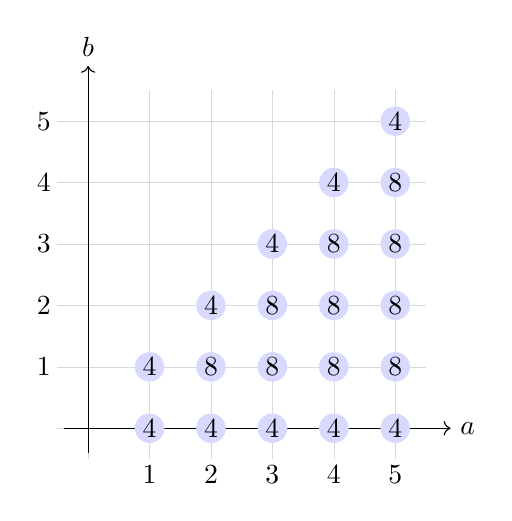
\begin{tikzpicture}[x=0.78cm,y=0.78cm]
\draw[step=1,gray!30,very thin] (-0.5,-0.5) grid (5.5,5.5);
\draw[->] (-0.4,0)--(5.9,0) node[right] {$a$};
\draw[->] (0,-0.4)--(0,5.9) node[above] {$b$};
\foreach \a in {1,...,5}{\foreach \b in {0,...,\a}{
 \ifnum\b=0\def\n{4}\else\ifnum\a=\b\def\n{4}\else\def\n{8}\fi\fi
 \fill[blue!15] (\a,\b) circle (0.24);
 \node at (\a,\b) {\n};}}
\foreach \k in {1,...,5}{\node[below] at (\k,-0.45){\k};\node[left] at (-0.45,\k){\k};}
\end{tikzpicture}
\caption{The 20 representatives $(-a,-b)$. Numbers are orbit sizes, not
search counts. The 10 boundary representatives have size four and the
10 interior representatives have size eight, covering all 120 normalized
first replies. A coordinate magnitude five also covers all larger actual
magnitudes of that coordinate.}
\label{fig:orbits}
\end{figure}

\section{Independent verification and observed computation}
\label{sec:compute}
\subsection{What the checker trusts}
The independent checker is an eight-source Python stack using the standard
library. It does not import the search implementation, the first checker,
RV2, or Rapfi. It reconstructs normalized axis insertions and five-segments
from finite sets; reconstructs the critical replies of symbolic rules;
checks the sequence sufficient conditions; and follows the complete
modular proof closure. At the opening layer it reconstructs $R$, checks
all 20 roots and all 120 representative assignments, validates each
symmetry matrix, and requires an empty-board interpretation.
Assertions must remain enabled; execution with Python's \code{-O} option
is rejected. A saved receipt is evidence of an earlier computation, not
a substitute for a fresh mathematical check in the final run.

The accepted empty cover has SHA-256
\begin{center}\small\ttfamily
fce6b466f2675cb5a76f40b1e979fb77bdfc4abc6971971510e1c60196adf85c.
\end{center}
The final recorded mathematical result has digest
\begin{center}\small\ttfamily
9720a055b970aa092dc216ca73059055d97d040ae3c47a31f357b26a7b40443b.
\end{center}
The final byte-closure audit has digest
\begin{center}\small\ttfamily
226562fd83b790dbce3f076aedad58e7ff22f9ec4d8da78fe29982cd448b90f4.
\end{center}
These digests identify frozen local records; they do not by themselves
provide access to those records. The complete proof-artifact repository
and its archival identifier have not yet been assigned.

\subsection{Completed run and scope of the statistics}
The final mathematical run checked all 20 opening roots and all 120
normalized first replies, with total bound 35 and no reused checked-file
receipts. The observed process exited with status zero. Across the 20 roots
there were 20 sequential four-worker pools, with 80 worker-process instances
in total, all observed exiting successfully. This is four concurrent
workers, not 80 concurrent workers. The fresh mathematical entry point
reported 27,837.450 seconds. The enclosing wrapper reported 27,837.498
seconds; the latter contains the former and they must not be added.

A separate complete byte audit read the selected dependency closure and
checked it against the fresh receipts. It reported 1,482,906 distinct
dependency paths and 1,652,612 file occurrences across roots, in
5,729.200 seconds. Distinct paths are not necessarily distinct contents.
The audit's actual process also exited with status zero. An operating-system
cache prefetch helper ran during that audit; each digest was still recomputed
from actual file bytes. Therefore this duration is not a cold-cache benchmark.

Table~\ref{tab:counts} records occurrences summed across opening roots.
Some subproofs are shared, so those sums differ from the distinct path union.
The node total is not the number of moves in a game or the number of
distinct infinite-board positions. These are observations of a particular
verified proof object, not lower bounds on certificate size.

\begin{table}[ht]
\centering
\begin{tabular}{lr}
\toprule Quantity & Observed value\\\midrule
Normalized first replies covered & 120\\
Symmetry representative roots checked & 20\\
Ordinary proof-file occurrences & 1,644,613\\
Ordinary reachable-node occurrences & 109,364,098\\
Bundle-file occurrences & 7,999\\
Bundle-edge occurrences & 1,954,756\\
Distinct selected dependency paths & 1,482,906\\
Fresh mathematical check, wall seconds & 27,837.450\\
Separate full byte audit, wall seconds & 5,729.200\\
\bottomrule
\end{tabular}
\caption{Recorded certificate and verification statistics. Occurrences can
repeat across roots. Mathematical phases, wrapper time, and audit time
are not independent CPU-cost measurements. No complete from-zero search
time or overall search speedup is inferred from these numbers.}
\label{tab:counts}
\end{table}

The machine currently reports an Intel Core i7-12700H with 20 logical
processors, Windows 11 Pro build 26200, about 31.7 GiB physical memory,
and Python 3.13.14. These observations were collected while preparing the
manuscript on 3 October 2026. They are current environment metadata, not
an independently recorded start-time environment of every historical
search. The verification's worker count is established by its actual run
records. A portable reproduction should record its own hardware, software,
actual exit status, and wall time.

\subsection{Failures and computational provenance}
Earlier unsuccessful runs are retained. One mathematical attempt failed
with a broken worker pool. One byte audit wrote a seal but its observed
process exited with status 120, so it was not accepted as the successful
final audit. A later audit failed with Windows error 5 while replacing a
progress file and produced no complete seal. The final reviewed audit
variant added only a bounded retry around progress-file replacement for
Windows sharing/access failures; the hashing and mathematical audit body
were unchanged. Persistent errors still cause failure. These failures are
execution provenance, not omitted proof branches, and are not added to the
successful-run timings as if they were successful computations.

The final small-record completion check binds the successful mathematical
run, byte audit, source digests, and actual roots. It is a record-integrity
gate, not a second full traversal of the mathematical proof. The eight
mathematical sources and selected proof bytes are unchanged by later
dashboard updates. Historical freezes of a much broader development tree
must not be described as the current hash of that whole tree after such
updates.

\begin{proof}[Proof of Theorem~\ref{thm:main}]
The completed independent run accepted the 20 representative-root
certificates, each with the specified rules, actual two-stone root,
and total-placement bound 35, and checked the 120 first-reply assignments.
The accepted short and long rules have the uniform strategy properties
proved in Sections~\ref{sec:short} and~\ref{sec:long}. By
Theorem~\ref{thm:sound}, each representative certificate wins from every
actual preimage within its remaining actual clock. Proposition~\ref{prop:opening}
then transports these strategies to every actual legal first reply after
Black starts at $(0,0)$. The 35 count includes those first two placements.
The byte audit binds this calculation to the selected actual proof bytes;
its record is an integrity witness for the finite computation, not an
additional mathematical assumption about distant play.
\end{proof}

\section{Search as an untrusted producer}
\label{sec:search}
Search generates candidates for the proof language. The producer uses
finite-board strategy suggestions, RV2 suggestions, Rapfi suggestions,
freestyle threat generation, and geometric move ordering. Engine outputs
are Black action proposals only. An exact-five engine can recommend a
move which is inappropriate when an overline wins, and a finite evaluation
window can omit relevant distant stones. Neither issue changes the target
rules: every proposed action must yield a proof accepted by the infinite
checker.

The final search mechanism is a persistent AND/OR computation. A Black
action is an OR choice among candidate actions but an AND obligation over
all its abstract outcomes. A White node is an AND obligation over all
abstract legal replies. Alternative Black actions retain separate child
sets; successes from different actions are never added to manufacture one
complete strategy. Completed candidate evaluations and accumulated budgets
are persisted so recovery does not repeatedly erase unfavorable trials.
Completed subproofs may be reused by the producer, whereas the final
independent check reconstructs the whole selected mathematical closure.

A search cutoff, exhausted candidate list, or incomplete task graph yields
UNKNOWN. It does not prove a White win or a Black loss. A White counterwin
against a particular Black proposal rejects that proposal, not every Black
strategy. The total count of 35 is a search and certificate bound chosen
for the exhibited strategy. There is no argument here that a valid Black
strategy cannot require a larger bound; the certificate proves that this
one does not.

Search time, recommendation time, database recovery, certificate writing,
mathematical verification, and byte auditing are different costs.
Historical runs include imports, interruptions, repairs, and experiments,
so a complete cold-start search cost for all 20 roots is presently unknown.
The manuscript consequently makes no claimed overall acceleration relative
to the $15\times15$ proof or to an earlier implementation. A speed claim
would require a controlled comparison of complete identical roots with
their proof and check costs.

\section{Reproducibility and publication preparation}
\label{sec:repro}
The proof object consists of the empty opening cover and its entire selected
dependency closure. A search database, dashboard, or collection of winning
example games cannot replace that closure. A release should contain:
\begin{enumerate}
\item the immutable cover, selected ordinary and bundle files, and a
 manifest binding their bytes;
\item the eight independent mathematical checker sources, plus a minimal
 standard-library entry point and usage instructions;
\item the sufficient-rule exposition, this manuscript, source and artifact
 versions, licenses, and declared research-tool contributions;
\item the successful-run records, with unsuccessful historical runs clearly
 distinguished from successful ones;
\item deterministic fresh-verification commands and a small quick example
 for checking installation, explicitly separate from the full proof.
\end{enumerate}
The search engines are not dependencies of the independent verification.
Publishing enough producer information to reproduce strategy generation
would be an additional reproducibility layer, not a logical premise of
checking the frozen certificate.

On the current workspace, the mathematical entry point is invoked as
\begin{quote}\small\ttfamily
python -B -m scripts.reference\_gap\_opening\_cover COVER\\
\hspace*{1em}--from-empty --workers 4 --output-dir NEW
\end{quote}
where COVER names the frozen cover and NEW is a previously unused directory.
The project documentation provides a wrapper which records source versions
before and after the run and supports a safe stop. A subsequent full byte
audit reads that new result and its dependency receipts. Both actual process
exit statuses must be checked. Assertions are enabled, old receipts are not
silently substituted, and a stopped or failed run is not an accepted result.
The byte audit is an archival integrity check in addition to the mathematical
check.

The current references include workspace-specific paths. Before public
release, they must be relocated or packaged so that every reference resolves
within a portable package. Rewriting a referenced file changes its digest
and all ancestors which bind that digest; it must not be described as a
byte-identical copy. Such a transformed release needs a new fresh full
verification and byte manifest. The accepted local originals remain
immutable. A path-resolving loader is another possible approach, but it
would be a new checker variant requiring review and independent
verification. This stage prepares the release design; it does not claim
that a portable transformed package has already passed that fresh check.

The complete selected logical byte size and compressed distribution size
are assessed separately in the accompanying artifact plan. A bounded,
non-random sample of 39 actual files comprised 5,050,297 payload bytes and
compressed to a 272,986-byte gzip tar archive (5.41\% of the sample payload).
It contained 20 opening-root headers, the cover, three further reachable
bundles, three ordinary plain-JSON DAGs, eight checker sources, and four
metadata records. Original byte digests were unchanged and archive members
round-tripped. The sample is incomplete and cannot be used to verify the
whole theorem. Full selected-closure and compressed release byte totals
remain unknown; this sample ratio is not extrapolated to them. Repository quotas and
licensing must be checked against the actual final package. This preprint does not claim that the complete proof artifact has already
been publicly archived or independently reproduced from a portable release.

The bounded path inspection found 1,460 referenced proof paths in the
sample, all relative, and Windows backslashes in the cover's path fields.
This is not an inventory of the entire dependency closure. On a POSIX
system, backslashes in such strings are not directory separators for
\code{pathlib}; a schema-aware portable derivation is therefore necessary
for at least those references. On Windows, preserving topology can avoid
some byte changes, but this does not establish relocatability of the
complete corpus. A release validation must run without access to the
original workspace. The eight mathematical source files total 73,668
bytes and need no third-party Python package; this compact verifier size
does not imply a compact certificate corpus.

\section{Discussion}
This result supplies a bounded strategy for the infinite strong freestyle
game. Its treatment of distant replies rests on complete insertion coverage
and explicitly checked sufficient rules. It is not based on a general
principle that distant stones are weak or can safely be ignored. A remote
White threat may cost Black actual defensive placements; the long-rule
clock accounts for them. Cases which fail the isolation or counterthreat
conditions require ordinary expansion rather than informal dismissal.

The abstraction is useful precisely because it is conservative. A
normalized state can represent several actual geometries and an action
can create several normalized children. Solving a stronger finite
obligation gives a strategy for all actual preimages. This also suggests a
tradeoff: coarse conservative states may enlarge proof trees. More
refined sufficient rules, alternative first-player actions, or more
compact formats could reduce proof size without changing the theorem,
but every such transformation needs a fresh soundness and verification
argument.

The remaining work concerns external review, portable artifact release,
and replication. It is separate from the completed local
computation. The 35-placement bound can be studied further, but neither
optimality nor a smaller universal remote-play bound is established here.

\appendix
\section{Opening-root statistics}
\label{app:stats}
{\small
\begin{longtable}{rrrrrr}
\caption{Selected opening-root observations from the completed fresh check. File and node counts are ordinary occurrences within each root; bundle files are separate. Seconds are the sum of that root's recorded header, mathematical-check, and binding phases, contained in the global wrapper time.}\label{tab:openings}\\
\toprule White representative & Orbit & Ordinary files & Nodes & Bundles & Seconds\\\midrule
\endfirsthead
\toprule White representative & Orbit & Ordinary files & Nodes & Bundles & Seconds\\\midrule
\endhead
$(-5,-5)$ & 4 & 163,582 & 7,532,881 & 442 & 4029.5\\
$(-5,-4)$ & 8 & 35,905 & 1,649,897 & 144 & 964.5\\
$(-5,-3)$ & 8 & 60,609 & 3,155,562 & 212 & 974.3\\
$(-5,-2)$ & 8 & 45,162 & 1,767,609 & 211 & 827.3\\
$(-5,-1)$ & 8 & 55,144 & 2,211,798 & 283 & 847.6\\
$(-5,0)$ & 4 & 113,174 & 6,199,978 & 585 & 2558.8\\
$(-4,-4)$ & 4 & 77,180 & 1,814,965 & 508 & 571.9\\
$(-4,-3)$ & 8 & 77,515 & 1,784,629 & 592 & 585.5\\
$(-4,-2)$ & 8 & 117,617 & 2,679,535 & 796 & 1836.5\\
$(-4,-1)$ & 8 & 74,006 & 2,844,235 & 531 & 514.3\\
$(-4,0)$ & 4 & 140,088 & 5,929,007 & 751 & 970.2\\
$(-3,-3)$ & 4 & 47,609 & 3,269,495 & 164 & 496.9\\
$(-3,-2)$ & 8 & 18,688 & 2,300,678 & 125 & 385.6\\
$(-3,-1)$ & 8 & 30,800 & 2,040,048 & 103 & 339.6\\
$(-3,0)$ & 4 & 11,529 & 1,967,360 & 80 & 298.8\\
$(-2,-2)$ & 4 & 15,807 & 2,152,198 & 112 & 338.9\\
$(-2,-1)$ & 8 & 21,678 & 3,477,398 & 143 & 548.4\\
$(-2,0)$ & 4 & 34,208 & 7,027,226 & 192 & 1308.0\\
$(-1,-1)$ & 4 & 499,165 & 36,834,514 & 1,973 & 8767.4\\
$(-1,0)$ & 4 & 5,147 & 12,725,085 & 52 & 664.8\\
\bottomrule
\end{longtable}
}


\section{Checker sources and byte identities}
\label{app:sources}
The following eight files are one independent checker stack, not eight
independent implementations of the whole theorem:
\begin{quote}\small\ttfamily
scripts/reference\_gap\_opening\_cover.py\\
scripts/reference\_gap\_bundle\_batched.py\\
scripts/reference\_gap\_bundle\_parallel.py\\
scripts/reference\_gap\_bundle\_verifier.py\\
scripts/reference\_gap\_verifier.py\\
scripts/reference\_infinite\_threat\_witness.py\\
scripts/reference\_prepared\_remote\_sequence.py\\
scripts/reference\_remote\_interruption\_sequence.py
\end{quote}
The publication inventory records their complete digests, the actual proof
roots, and the completed mathematical and byte-audit records. Digest checks
are necessary for identifying the verified version; they do not authenticate
an observer or establish mathematical correctness by themselves.

\section{Research-tool disclosure and artifact availability}
The project used OpenAI Codex with language-model assistance for research
exploration, software development, debugging, and manuscript preparation.
RV2 and Rapfi were used as untrusted move advisers during strategy search.
Their evaluations and suggested moves were not proof acceptance criteria.
The mathematical checker reconstructs the required successor coverage and
verifies the complete selected certificate closure without importing the
search implementation or either move-advice engine. Exact language-model
version identifiers are not established for every historical interaction.

The named author provided the research objective, strategic guidance, and
project supervision. This preprint reports the completed local independent
verification documented in the paper; it has not undergone external peer
review. Proof-assistant formalization is not part of the result.

This release contains the manuscript only. At the time of this version,
the complete certificate corpus and a relocatable public verification
package are not publicly available. Readers cannot yet reproduce the
full computation from the publicly released material. The certificate
corpus, checker package, byte manifest, and portable verification
instructions are planned as a separate artifact release. Packaging and
fresh verification in an environment without access to the original
workspace remain future work. No completion date or archive identifier
is asserted in this version.

\begin{thebibliography}{99}
\bibitem{Allis1993} L. V. Allis, H. J. van den Herik, and M. P. H. Huntjens.
Go-Moku solved by new search techniques. AAAI Fall Symposium on Games:
Planning and Learning, 1993.
\bibitem{Allis1996} L. V. Allis, H. J. van den Herik, and M. P. H. Huntjens.
Go-Moku solved by new search techniques. Computational Intelligence
12(1) (1996), 7--23.
\url{https://doi.org/10.1111/j.1467-8640.1996.tb00250.x}.
\bibitem{Erde2012} J. Erde. An $n$-in-a-row game.
arXiv:1209.5123v1, 2012.
\url{https://arxiv.org/abs/1209.5123}.
\bibitem{Hefetz2014} D. Hefetz, M. Krivelevich, M. Stojakovi\'c, and T. Szab\'o.
Positional Games. Oberwolfach Seminars 44, Birkh\"auser, 2014.
\url{https://doi.org/10.1007/978-3-0348-0825-5}.
\bibitem{Gyorffy2019} L. Gy\H{o}rffy, G. Makay, and A. Pluh\'ar.
The pairing strategies of the 9-in-a-row game.
Ars Mathematica Contemporanea 16(1) (2019), 97--109.
\url{https://doi.org/10.26493/1855-3974.1350.990}.
\bibitem{Pluhar2022} A. S. Pluh\'ar. One and two-person Positional games.
Dissertation submitted to the Hungarian Academy of Sciences for the title
MTA Doktora, Szeged, title-page date 2022; deposited in REAL-d in 2023.
\url{https://real-d.mtak.hu/1545/}.
\bibitem{Hamkins2023} J. D. Hamkins and D. Leonessi.
Infinite Hex is a draw. Integers 23 (2023), G6.
\url{https://doi.org/10.5281/zenodo.10075843}.
\end{thebibliography}
\end{document}
